\section{Throughput benchmark}

We verified our performance goal by running \ac{SCITE} and \ac{ffSCITE} in different configurations and comparing their makespan. Three dimensions may impact the makespan of the \ac{SCITE} algorithm: The input size, i.e. the number of cells and genes included in the input, the number of chains to execute, and the number of steps to execute per chain. We used three random inputs, one with 16 cells and 15 genes, one with 32 cells and 31 genes, and one with 64 cells and 63 genes. Our options for the number of chains were 6 and 12, and we used all chain lengths from 500,000 steps to 2,000,000 steps in increments of 500,000 steps. We also let every application run ten times for every parameter combination and averaged out the resulting makespan. We should also note that \ac{ffSCITE} measures the makespan of the \ac{FPGA} kernels and therefore excludes the time to read inputs, generate initial states and emit the resulting tree. \ac{SCITE} however measures the runtime of the entire application, which introduces some noise to the measurements, especially for small parameters. However, these effects should be negligible for big parameters.

The resulting performance metrics are plotted in figure \ref{fig:performance}. \ac{ffSCITE}'s throughput remains constant for all parameter combinations, as we have predicted. Therefore, \ac{ffSCITE}'s graphs are dashed lines since they would otherwise overlap. The exact throughput of \ac{ffSCITE} is 566.72 ksteps/s, which is 98.1\% of the performance we predicted. An additional profiling run using Intel VTune also reveals that the loop with the highest occupation with 99.8\% is the Tree Scorer loop, again as predicted. The next most-occupied loops are the other internal loops of the tree scorer with 14.0\%, which roughly matches the anticipated occupation of $\frac{512}{64} = 12.5\%$. We therefore still consider our model a match since we generally see the predicted behavior, within some errors.

The performance metrics of \ac{SCITE} however have more variation than \ac{ffSCITE}, which is expected: It only iterates through its loops as often as necessary, which means that the throughput of \ac{SCITE} in steps per second is bigger for smaller inputs. There is also some noise in the measurements, both due to the previously mentioned measurement scope as well as warming caches and interactions with the operating system. One effect that we however do not and do not try to understand is that for the small input, \ac{SCITE}'s throughput appears to decrease with an increasing number of steps. However, the throughput is nearly constant for the mid-sized and big input and we can therefore reliably deduce that \ac{ffSCITE} has an up to 8.53 times higher throughput than \ac{SCITE}. It might also be interesting to further explore the effects of different input sizes and chain counts. However, this would require an in-depth analysis of \ac{SCITE}'s performance, which is outside the scope of this thesis.

\todo[inline]{Give information about \ac{SCITE} benchmark setup (compiler flags etc.)}

\begin{figure}
    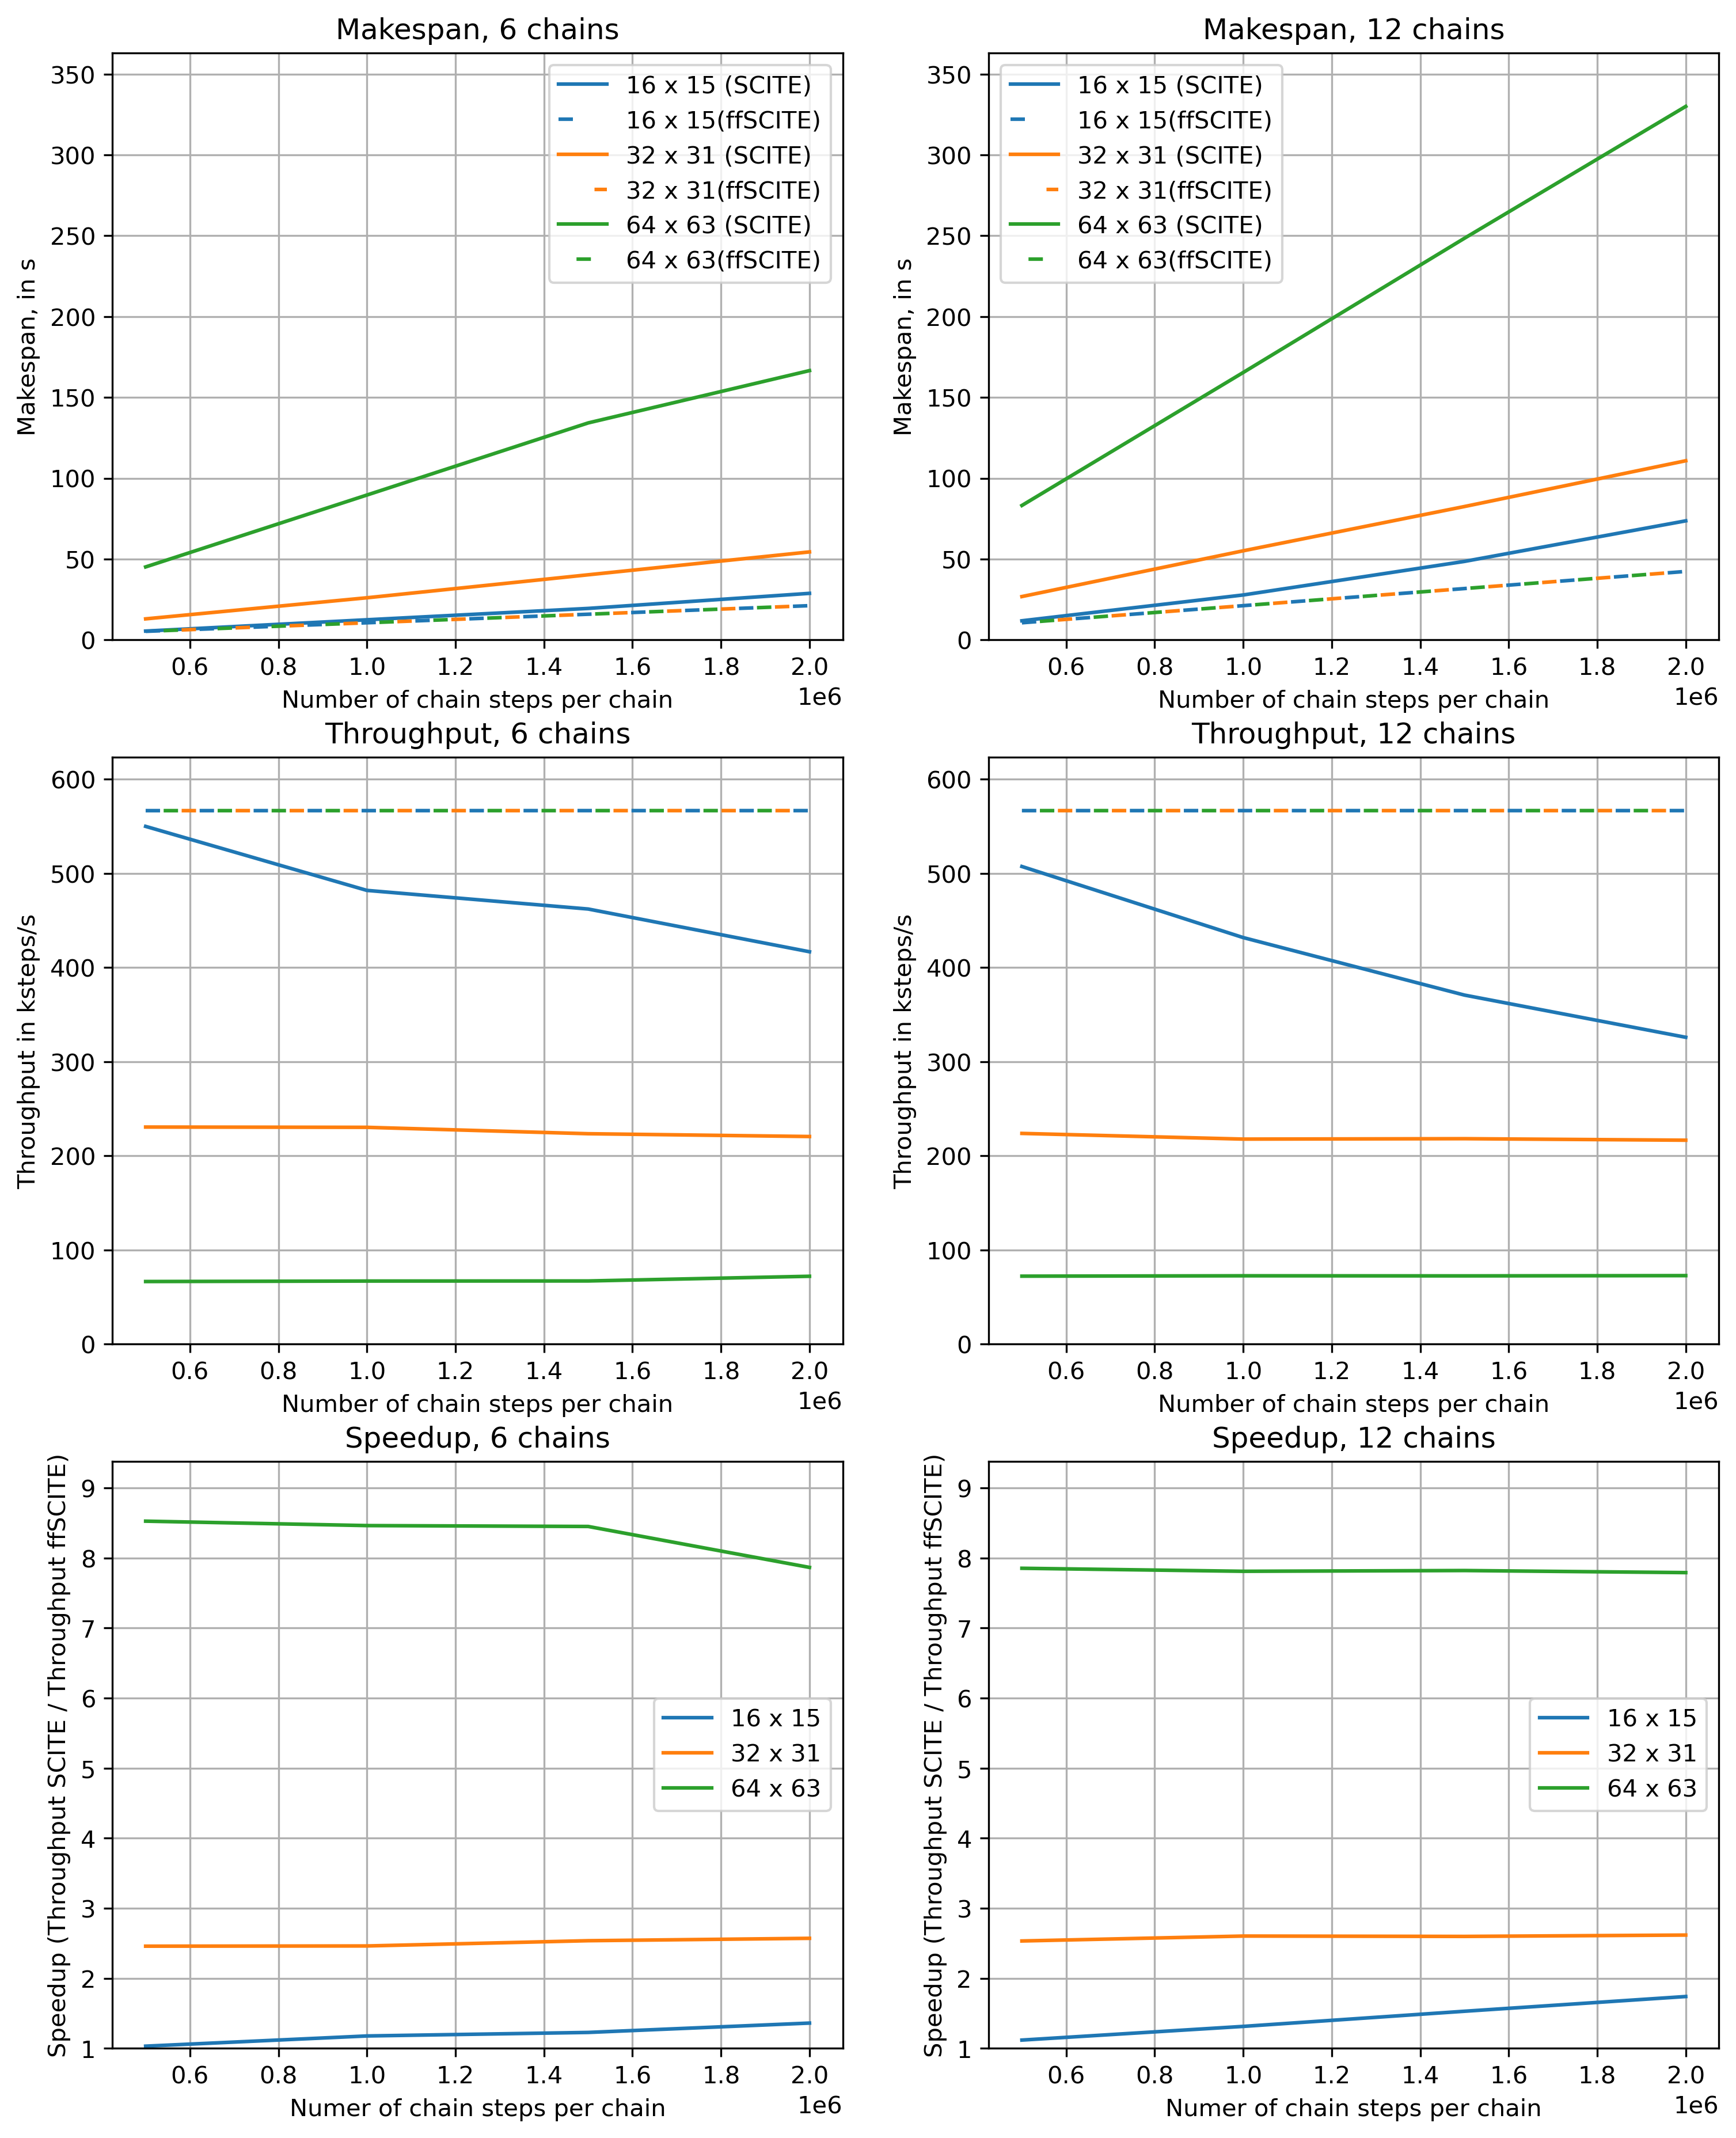
\includegraphics[width=\textwidth]{figures/performance.png}
    \caption{Performance metrics of \ac{ffSCITE} and \ac{SCITE}. The colors indicate the input size, while the dashed lines indicate \ac{ffSCITE}'s metrics and the solid lines indicate \ac{SCITE}'s metrics. The speedup graphs indicate \ac{SCITE}'s makespan divided by \ac{ffSCITE}'s makespan for the respective inputs.}
    \label{fig:performance}
\end{figure}

We had also set ourselves the optional goal to obtain a higher throughput than Ernst et al. \cite{ernst2020Performance}. We were not able to properly verify this since we neither have access to their source code nor did they list absolute performance figures or the total single-thread speedup compared to the reference implementation. However, we assume that their throughput is higher since their first single-threaded optimization alone achieved a speedup of 6.4 compared to the reference and they were able to use multiple threads to increase their throughput by a factor of 61.3 compared to their single-threaded throughput.